% arara: pdflatex
% !arara: animate: {delay: 80}
% !arara: indent: {overwrite: yes, localSettings: yes}
\documentclass[mathserif, 14pt, xcolor=svgnames]{beamer}
%%%%%%%%%%%%%%%%%%%%%%%%%%%%%%%%%%%%%%%%%%%%%%%%%%%%%%%%%%%%%%%%%%%%%%%%%%%%%%
% \embedvideo{<poster or text>}{<video file (MP4+H264)>}
% \embedvideo*{...}{...}                     % auto-play
%%%%%%%%%%%%%%%%%%%%%%%%%%%%%%%%%%%%%%%%%%%%%%%%%%%%%%%%%%%%%%%%%%%%%%%%%%%%%%

\usepackage[bigfiles]{pdfbase}
\ExplSyntaxOn
\NewDocumentCommand\embedvideo{smm}{
  \group_begin:
  \leavevmode
  \tl_if_exist:cTF{file_\file_mdfive_hash:n{#3}}{
    \tl_set_eq:Nc\video{file_\file_mdfive_hash:n{#3}}
  }{
    \IfFileExists{#3}{}{\GenericError{}{File~`#3'~not~found}{}{}}
    \pbs_pdfobj:nnn{}{fstream}{{}{#3}}
    \pbs_pdfobj:nnn{}{dict}{
      /Type/Filespec/F~(#3)/UF~(#3)
      /EF~<</F~\pbs_pdflastobj:>>
    }
    \tl_set:Nx\video{\pbs_pdflastobj:}
    \tl_gset_eq:cN{file_\file_mdfive_hash:n{#3}}\video
  }
  %
  \pbs_pdfobj:nnn{}{dict}{
    /Type/RichMediaInstance/Subtype/Video
    /Asset~\video
    /Params~<</FlashVars (
      source=#3&
      skin=SkinOverAllNoFullNoCaption.swf&
      skinAutoHide=true&
      skinBackgroundColor=0x5F5F5F&
      skinBackgroundAlpha=0
    )>>
  }
  %
  \pbs_pdfobj:nnn{}{dict}{
    /Type/RichMediaConfiguration/Subtype/Video
    /Instances~[\pbs_pdflastobj:]
  }
  %
  \pbs_pdfobj:nnn{}{dict}{
    /Type/RichMediaContent
    /Assets~<<
      /Names~[(#3)~\video]
    >>
    /Configurations~[\pbs_pdflastobj:]
  }
  \tl_set:Nx\rmcontent{\pbs_pdflastobj:}
  %
  \pbs_pdfobj:nnn{}{dict}{
    /Activation~<<
      /Condition/\IfBooleanTF{#1}{PV}{XA}
      /Presentation~<</Style/Embedded>>
    >>
    /Deactivation~<</Condition/PI>>
  }
  %
  \hbox_set:Nn\l_tmpa_box{#2}
  \tl_set:Nx\l_box_wd_tl{\dim_use:N\box_wd:N\l_tmpa_box}
  \tl_set:Nx\l_box_ht_tl{\dim_use:N\box_ht:N\l_tmpa_box}
  \tl_set:Nx\l_box_dp_tl{\dim_use:N\box_dp:N\l_tmpa_box}
  \pbs_pdfxform:nnnnn{1}{1}{}{}{\l_tmpa_box}
  %
  \pbs_pdfannot:nnnn{\l_box_wd_tl}{\l_box_ht_tl}{\l_box_dp_tl}{
    /Subtype/RichMedia
    /BS~<</W~0/S/S>>
    /Contents~(embedded~video~file:#3)
    /NM~(rma:#3)
    /AP~<</N~\pbs_pdflastxform:>>
    /RichMediaSettings~\pbs_pdflastobj:
    /RichMediaContent~\rmcontent
  }
  \phantom{#2}
  \group_end:
}
\ExplSyntaxOff
%%%%%%%%%%%%%%%%%%%%%%%%%%%%%%%%%%%%%%%%%%%%%%%%%%%%%%%%%%%%%%%%%%%%%%%%%%%%%%
%\documentclass[handout,mathserif]{beamer}
\usepackage{physics, amsmath,amsfonts,amsthm,amssymb, mathtools,steinmetz, gensymb, siunitx}	
\usepackage{caption}
%\usepackage{setspace}
\usepackage{pgf,tikz,pgfplots,wrapfig}
\usepackage{rotating}
\usepackage{fancyhdr}
\usepackage{float}
\usepackage{listings}
\usepackage{array}
\usepackage{booktabs,multirow}
\usepackage{bm}
\usepackage{url}  % to handle urls
\usepackage[comma,authoryear]{natbib}  % for authordate ref style --  allows \citet (textual), and \citep (parenthesized)
\usepackage{hyperref}
\usepackage{pifont}


\newcommand{\tfont[1]}{ #1}

\renewcommand {\cite} {\citep}  % default for cite is citet in natbib - so change it
\renewcommand\bibname{References}    % if not using newrucsthesis sty file
\bibpunct[, ]{(}{)}{;}{a}{,}{,}

\renewcommand {\thempfootnote} {\arabic{mpfootnote}}  % default for cite is citet in natbib - so change it

\usetikzlibrary{positioning}
\usetikzlibrary{fit}
\usetikzlibrary{backgrounds}
\usetikzlibrary{calc}
\usetikzlibrary{shapes}
\usetikzlibrary{mindmap}
\usetikzlibrary{decorations.text}
\pgfplotsset{compat=1.7}
\usepackage{tikz}

\definecolor{coolblack}{rgb}{0.0, 0.18, 0.39}
\definecolor{OxfordBlue}{rgb}{0.0, 0.082, 0.21}
\definecolor{Tangerine}{rgb}{0.95, 0.52, 0.0}
\definecolor{Tangelo}{rgb}{0.98, 0.35, 0.0}

\newcommand\blfootnote[1]{
  \begingroup
  \renewcommand\thefootnote{}\footnote{#1}
  \addtocounter{footnote}{-1}
  \endgroup
}
%\renewcommand*{\bibfont}{\tiny}

\newcommand{\topline}{%
  \tikz[remember picture,overlay] {%
    \draw[Tangerine,ultra thick] ([yshift=-1.6em]current page.north west)-- ([yshift=-1.6em,xshift=\paperwidth]current page.north west);}}

\addtobeamertemplate{frametitle}{}{\topline%
}

% tikzmark command, for shading over items
\newcommand{\tikzmark}[1]{\tikz[overlay,remember picture] \node (#1) {};}

\setbeamercolor{frametitle}{fg=white}

% title color
\setbeamercolor{title}{fg=white}
\setbeamercolor{footnote mark}{fg=.}
\setbeamercolor{normal text}{fg=white}

% standard enumeration
\setbeamertemplate{enumerate items}{(\arabic{enumi})}

% color of slides
\setbeamercolor{background canvas}{bg=OxfordBlue}

% color of references
\setbeamercolor{bibliography item}{fg=white}
\setbeamercolor{bibliography entry title}{fg=white}
\setbeamercolor{bibliography entry author}{fg=white}
\setbeamercolor{bibliography entry date}{fg=white}
\setbeamercolor{bibliography entry note}{fg=white}
\setbeamercolor{bibliography entry url}{fg=white}
\setbeamercolor{bibliography entry organiation}{fg=white}
\setbeamercolor{bibliography entry location}{fg=white}
%
%\setbeamerfont{bibliography item}{size=\tiny}
%\setbeamerfont{bibliography entry title}{size=\tiny}
%\setbeamerfont{bibliography entry author}{size=\tiny}
%\setbeamerfont{bibliography entry date}{size=\tiny}
%\setbeamerfont{bibliography entry note}{size=\tiny}
%\setbeamerfont{bibliography entry url}{size=\tiny}
%\setbeamerfont{bibliography entry organization}{size=\tiny}
%\setbeamerfont{bibliography entry location}{size=\tiny}
%
% default itemize
\setbeamertemplate{itemize items}[circle]

% no navigation symbols
\setbeamertemplate{navigation symbols}{}

\setbeamercolor{itemize item}{fg=Tangelo}
\setbeamertemplate{itemize item}{\maltese}
\setbeamercolor{itemize subitem}{fg=Tangelo}
\setbeamertemplate{itemize subitem}{\begin{rotate}{90}$\diamondsuit$\end{rotate}}

\usepackage[T1]{fontenc}
%\usepackage{fontspec}
%\setmainfont{TeX Gyre Pagella}%% The Palatino from the TeX Gyre Project

% transparency
\setbeamercovered{invisible}

% for resuming lists across frames
\newcounter{savedenum}
\newcommand*{\saveenum}{\setcounter{savedenum}{\theenumi}}
\newcommand*{\resume}{\setcounter{enumi}{\thesavedenum}}

% title
\title{Tracking and Detection of Multiple Human Faces }
\subtitle{}

\author[Gouws]{J L Gouws\inst{1}\\[1ex]  \and {\small Supervisor: Mr. J Connan\inst{1}}}
\date{\today}
\institute[RU]{\inst{1} Rhodes University}
\tikzset{
   invisible/.style={opacity=0},
   visible on/.style={alt=#1{}{invisible}},
   alt/.code args={<#1>#2#3}{%
      \alt<#1>{\pgfkeysalso{#2}}{\pgfkeysalso{#3}} % \pgfkeysalso doesn't change the path
   },
}

%\includeonlyframes{daytoday}

\begin{document}

\begin{frame}
   \maketitle
\end{frame}

\usetikzlibrary{shapes.geometric, arrows}

\tikzstyle{startstop} = [draw, line width = 0.2em, fill = white, rectangle, rounded corners, minimum width=3cm, minimum height=1cm,text centered, text = black]
\tikzstyle{io} = [draw, line width = 0.2em, text = black, trapezium, trapezium left angle=70, trapezium right angle=110, minimum width=3cm, minimum height=1cm, text centered, draw=black]
\tikzstyle{process} = [draw, line width = 0.2em, text = black, rectangle, minimum width=3cm, minimum height=1cm, text centered, draw=black]
\tikzstyle{decision} = [diamond, aspect = 2.5,minimum width=2cm, minimum height=0.5cm, text centered, draw=black]
\tikzstyle{arrow} = [line width = 0.2em,->,>=stealth]
\tikzstyle{line} = [thick]

\bgroup
\begin{frame}{Presentation Overview}
  \centering
  \begin{tikzpicture}[node distance=3em]
    \pause
    \node (ps) [startstop, draw = Chartreuse, fill = Chartreuse!10] {Problem Statement};
    \pause
    \node (litRev) [io, draw = Salmon, fill = Salmon!20, below of=ps] {Literature Review};
    \draw[arrow] (ps) -- (litRev);
    \pause
    \node (progress) [process, draw = Goldenrod, fill = Goldenrod!20, below of=litRev] {Progress};
    \draw[arrow] (litRev) -- (progress);
    \pause
    \node (future) [io, draw = DarkSeaGreen, fill = DarkSeaGreen!20, below of=progress] {Going Foward};
    \draw[arrow] (progress) -- (future);
    \pause
    \node (qs) [startstop, draw = Red, fill = Red!30, below of=future] {Questions};
    \draw[arrow] (future) -- (qs);

  \end{tikzpicture}
\end{frame}
\egroup

\bgroup
\begin{frame}{Problem Statement}
  \begin{minipage}[t]{\textwidth}
  { \Large
    The design and implementation of a long-term tracking system\pause--given minimal input data,
    the system can count the number and measure the duration of appearances of multiple
    target faces in a single video stream\pause--can use the TLD\footnotemark[1] framework.
  }
  \end{minipage}
  \footnotetext[1]<3->{\citep{KalalPHD}}
\end{frame}
\egroup


\bgroup

\begin{frame}{Short-term Tracking Challenges}
    \begin{itemize}
      \setlength\itemsep{1.5em}
       \item \hspace{0pt}
         \pause Class agnostic
       \item \hspace{0pt}
         \pause Deformations
       \item \hspace{0pt}
         \pause Lighting condition changes
       \item \hspace{0pt}
          \pause Occlusions
    \end{itemize}
\end{frame}
\egroup

\bgroup
\begin{frame}{SiamFC}
   \begin{itemize}
     \setlength\itemsep{1.2em}
     \item \hspace{0pt}
       \pause \citet{bertinetto2016}s' solution
     \item \hspace{0pt}
       \pause Fully-Convolutional 
     \item \hspace{0pt}
       \pause Siamese Neural Networks
      \begin{center}
        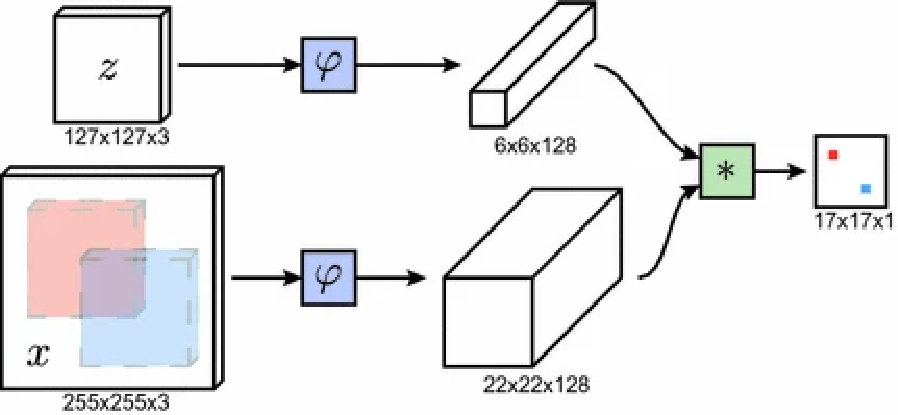
\includegraphics[scale=0.5]{convSiamese.pdf}
      \end{center}
    \end{itemize}
\end{frame}
\egroup

\bgroup
\begin{frame}{Short-term Tracking Approaches}

    \begin{itemize}
      \setlength\itemsep{1.2em}
       \item \hspace{0pt}
         Discriminative Single Shot tracker \citep{lukezic2020} 
         \begin{center}
          \raisebox{-.5\height}{\embedvideo*{\includegraphics[width = 0.30 \textwidth]{D3S.jpg}}{D3S.mp4}}
         \end{center}
       \item \hspace{0pt}
          Multi-Domain CNNs \citep{Nam2016}
       \item \hspace{0pt}
         SiamMask \citep{wang2019}
          \begin{itemize}
            \item VPUSiamM \cite{VOT2020}
            \item RPT
            \item OceanPlus
          \end{itemize}
    \end{itemize}
\end{frame}
\egroup

\bgroup
\begin{frame}{Long-term Tracking Challenges}
    \begin{itemize}
      \setlength\itemsep{1.5em}
       \item \hspace{0pt}
         \pause Perform short-term tracking 
       \item \hspace{0pt}
         \pause Determine tracker failure
       \item \hspace{0pt}
          \pause Re-detect target
          \begin{itemize}
            \setlength\itemsep{1.5em}
             \item \hspace{0pt}
               \pause
                ST tracker not initialized on target
          \end{itemize}
       \item \hspace{0pt}
          \pause Tracker Drift
    \end{itemize}
\end{frame}
\egroup

\bgroup
\begin{frame}{Long-term Tracking Approaches}
  \begin{itemize}
      \setlength\itemsep{1.3em}
      \setlength\itemindent{0em}
       \item \hspace{0pt}
         Combinations of tracking systems
       \item \hspace{0pt}
         Base short-term tracker
       \item \hspace{0pt}
         Re-detection mechanism
       \item \hspace{0pt}
         Verifier
       \item \hspace{0pt}
         LTD-SE 
          \begin{itemize}
            \setlength\itemindent{-0.5em}
             \item \hspace{0pt}
               Short-term: Extended Resnet and SiamMask
             \item \hspace{0pt}
               Re-detection: BB regression \citep{girshick2014}
             \item \hspace{0pt}
               MDNet based verifier
           \end{itemize}
    \end{itemize}
\end{frame}
\egroup

\bgroup
\begin{frame}{Implementation}
    \begin{itemize}
      \setlength\itemsep{1.5em}
       \item \hspace{0pt}
         \pause C++ code base 
       \item \hspace{0pt}
         \pause Object Oriented
          \begin{itemize}
            \setlength\itemsep{0.5em}
             \item \hspace{0pt}
               \pause Simple Interface
             \item \hspace{0pt}
               \pause Over-engineered
          \end{itemize}
       \item \hspace{0pt}
          \pause Dynamic library
    \end{itemize}
\end{frame}
\egroup


\begin{frame}{Progress Demonstration}
  \begin{center}

    Intel(R) Core(TM) i7-8550U CPU @ 1.80GHz\\
    640\texttimes 360p\\
    \vskip 1em

    \begin{minipage}[t]{0.48\textwidth}
      \begin{center}
        DCF \footnotemark[2]\\
        16.9 FPS
        \embedvideo*{\includegraphics[width=\textwidth]{tldDCF.jpg}}{tldDCF.mp4}
      \end{center}
    \end{minipage}
    \begin{minipage}[t]{0.48\textwidth}
      \begin{center}
        KCF \footnotemark[2]\\
        16.5 FPS
        \embedvideo*{\includegraphics[width=\textwidth]{tldKCF.jpg}}{tldKCF.mp4}
      \end{center}
    \end{minipage}
  \end{center}
  \footnotetext[2]{\citep{Enriques2014}}
\end{frame}

\begin{frame}[label=deliverables]{Deliverables}
  \begin{itemize}
    \setlength\itemsep{1.2em}
     \item 
        \pause Finding public videos
          \pause \textcolor{orange}{ \ding{51}}\textsuperscript{\textcolor{orange}{\kern-0.56em\small\ding{55}}}
     \item 
        \pause Full Implementation of Predator
          \pause \textcolor{orange}{ \ding{51}}\textsuperscript{\textcolor{orange}{\kern-0.56em\small\ding{55}}}
          %\pause 
        \pause \item Integrating KCF and DCF \pause \textcolor{green}{ \ding{51}}
        \pause \item Reviewing VOT \pause \textcolor{green}{ \ding{51}}
        \pause \item Investigating Random Ferns \pause \textcolor{red}{ \ding{55}}
  \end{itemize}
\end{frame}

\bgroup
\begin{frame}{Future Focus}
    \begin{itemize}
      \setlength\itemsep{1.4em}
       \item \hspace{0pt}
         \pause Stable learning
          \begin{itemize}
            \setlength\itemsep{1.4em}
             \item \hspace{0pt}
               \pause Refer to MATLAB code
          \end{itemize}
       \item \hspace{0pt}
         \pause Multiple face extension
          \begin{itemize}
            \setlength\itemsep{1.4em}
             \item \hspace{0pt}
               \onslide<5->{ICA \citep{ICAFaceRecog}}
             \item \hspace{0pt}
               \onslide<5->{Multiple pose \citep{viewBasedFaceRecog}}
          \end{itemize}
          \pause
       \item \hspace{0pt}
         \pause \onslide<6->{Complete thesis}
          \begin{itemize}
            \setlength\itemsep{1.4em}
             \item \hspace{0pt}
               \pause \onslide<7->{Parallel with implementation}
             \item \hspace{0pt}
               \pause \onslide<8->{Amdahl's Law?}
          \end{itemize}
    \end{itemize}
\end{frame}
\egroup

\bgroup
\begin{frame}[label=extensionMethods]
  \frametitle{Extension Methods}

      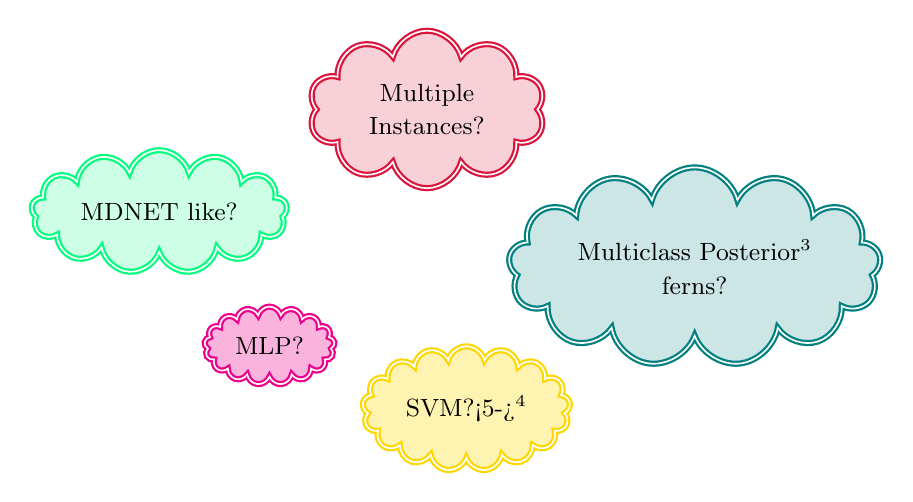
\begin{tikzpicture}[every node/.append style={cloud,draw,thick,align=center}]
        \onslide<2->{
            \node[draw=Crimson,double,fill=Crimson!20, minimum width=3cm,minimum height=2cm,cloud puffs=10, aspect=1.8, text = black] at (0,0.3) {\small Multiple\\ \small Instances?};
          }
        \onslide<3->{
            \node[draw=teal,double,cloud,fill=teal!20, cloud puffs=13, aspect=2.6, text = black] at (3.4, -1.7) {\small Multiclass Posterior\footnotemark[3]\\ \small ferns?};
          }
        \onslide<4->{
            \node[draw=Gold,double, fill=Gold!30, minimum height=3em, minimum width=5em,cloud puffs=17, aspect=2, text = black] at (0.5, -3.5) {\small SVM?\only<5->{\footnotemark[4]}};
          }
          \onslide<6->{
            \node[draw=magenta,double, fill=magenta!30, minimum height=2.5em, cloud puffs=17, aspect=2, text = black] at (-2, -2.7) {\small MLP?};
          }
          \onslide<7->{
            \node[draw=SpringGreen,double, fill=SpringGreen!20, cloud puffs=13, aspect=3.1, text = black] at (-3.4, -1) {\small MDNET like?};
          }
%         \pause
%            \node[draw=orange,double,above=0.5cm of Animals, fill=orange!30, minimum width=2cm,minimum height=1cm,cloud puffs=13, aspect=0.9]{...?};
      \end{tikzpicture}
    \footnotetext[3]<3->{\citep{murphy2012}}
    \footnotetext[4]<5->{Pegasos \citep{shalev2011}}

\end{frame}
\egroup

\begin{frame}{References}
    \bibliographystyle{ruauthordate}
    \fontsize{6pt}{6pt}\selectfont
%    { \tiny
    \bibliography{references.bib}   	% load in the citation info from ref.bib
%    }
\end{frame}

\end{document}


%\iffalse
 %  \begin{columns}
 %     \begin{column}[t]{.65\textwidth}
 %        What tools do faculty use?
 %
 %        \begin{tikzpicture}[every node/.append style={align=center}]
 %           \begin{pgfonlayer}{background}
 %              \node[circle,fill=red!30,draw=black,thick,minimum size=5cm](0,0){Microsoft Word\\ 86\%};
 %           \end{pgfonlayer}{background}
 %           \pause
 %              \visible<2->{\filldraw[gray,opacity=0.5] (2.5,0) arc (0:-190:2.5cm) -- (0,0)node[black,opacity=1,anchor=north east,scale=1,inner sep=.5cm] {MathType \\ 60\%};}
 %           \pause
 %              \visible<3->{\node[circle,fill=blue!40,draw=black,scale=1.15] at (2.3,-1){\LaTeX\\16\%};}
 %           \pause
 %              \visible<4->{\node[circle,fill=orange!40,draw=black,scale=0.65] at (2.3,1){Open Office\\12\%};}
 %        \end{tikzpicture}
 %     \end{column}%
 %\fi

\begin{frame}{Rule of four}

   \centering
   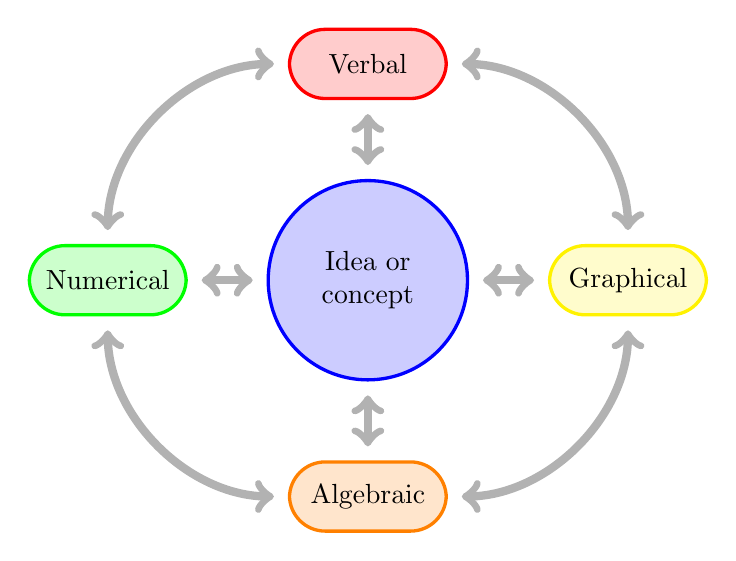
\begin{tikzpicture}[approach/.style={draw,very thick, fill=blue!20, text width=5em,
            text centered, minimum height=2.5em,rounded corners=3ex},
         idea/.style={draw, very thick,fill=blue!40, circle,text width=6em,
            text centered, minimum height=2.5em},
         connections/.style={<->,draw=black!30,line width=3pt,shorten <=5pt,shorten >=5pt},
      ]

      % Draw diagram elements
      \node (idea) [idea,draw=blue,fill=blue!20]  {Idea or concept};
      \pause
         \node (verbal) [approach,draw=red,fill=red!20,above=of idea]  {Verbal};
         \node (tabular) [approach,draw=green,fill=green!20,left=of idea]  {Numerical};
         \node (graphical)[approach,draw=yellow,fill=yellow!20,right=of idea] {Graphical};
         \node (formular)[approach,draw=orange,fill=orange!20,below=of idea] {Algebraic};

         % Draw arrows between elements
         \draw[connections] (idea) -- (formular) ;
         \draw[connections] (idea) -- (verbal);
         \draw[connections] (idea) -- (graphical);
         \draw[connections] (idea) -- (tabular);
         \draw[connections] (verbal.west) to[out=180,in=90](tabular.north) ;
         \draw[connections] (verbal.east) to[out=0,in=90](graphical.north) ;
         \draw[connections] (tabular.south) to[out=-90,in=180](formular.west) ;
         \draw[connections] (graphical.south)to[out=-90,in=0](formular.east);
   \end{tikzpicture}

\end{frame}

\begin{frame}[label=workflow]{Workflow}

   \makebox[\textwidth][c]{%
      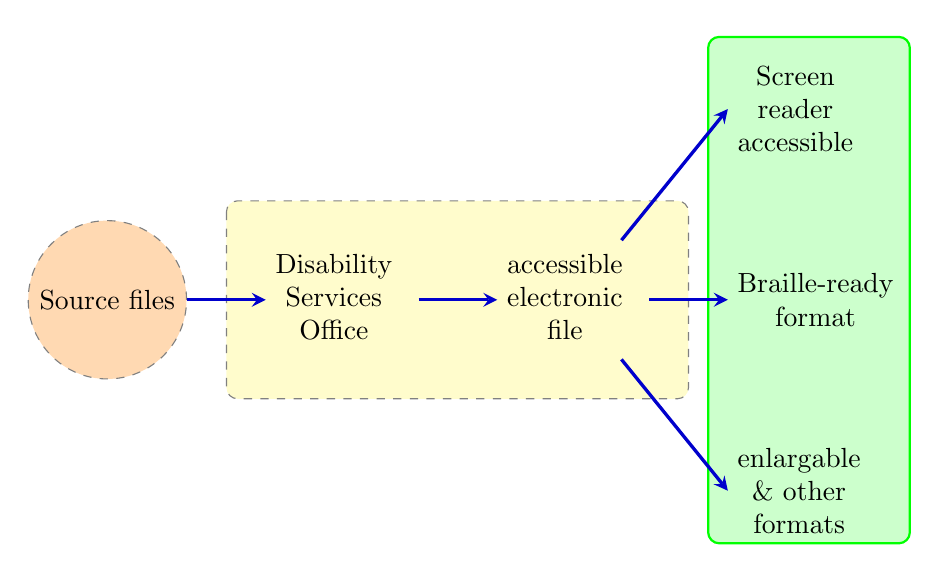
\begin{tikzpicture}[
            outpt/.style={->,blue!80!black,very thick},
            >=stealth,
         every node/.append style={align=center}]
         \node (kaela) at (0,0) {\begin{tabular}{@{}c}Disability\\ Services \\ Office \end{tabular}};
         \pause
            \node (accessfile) [right=of kaela] {\begin{tabular}{@{}c}accessible\\ electronic \\ file \end{tabular}};
            \draw[outpt](kaela)--(accessfile);
            % Draw background
            \begin{pgfonlayer}{background}
               % Left-top corner of the background rectangle
               \path (kaela.west |- kaela.north)+(-0.5,0.5) node (a) {};
               % Right-bottom corner of the background rectanle
               \path (accessfile.east |- accessfile.south)+(+0.5,-0.5) node (c) {};
               % Draw the background
               \path[fill=yellow!20,rounded corners, draw=black!50, dashed]
               (a) rectangle (c);
            \end{pgfonlayer}
         \pause
            \node (screen)[above right=of accessfile]{Screen\\ reader\\ accessible};
            \node (braille)[right =of accessfile]{Braille-ready\\ format};
            \node (enlarge)[below right=of accessfile]{enlargable\\ \& other \\ formats};
            \draw[outpt](accessfile)--(screen.west);
            \draw[outpt](accessfile)--(braille);
            \draw[outpt](accessfile)--(enlarge.west);
            \begin{pgfonlayer}{background}
               % Left-top corner of the background rectangle
               \path (screen.west |- screen.north)+(-0.25,0.25) node (a) {};
               % Right-bottom corner of the background rectanle
               \path (enlarge.east |- enlarge.south)+(0.5,0) node (c) {};
               % Draw the background
               \path[fill=green!20,rounded corners, draw=green,thick]
               (a) rectangle (c);
            \end{pgfonlayer}
         \pause
            \node (source) [left=of kaela,draw=black!50,dashed,circle,fill=orange!30]{Source files};
            \draw[outpt](source)--(kaela);
      \end{tikzpicture}
   }
\end{frame}

\begin{frame}{Stand alone concept}

   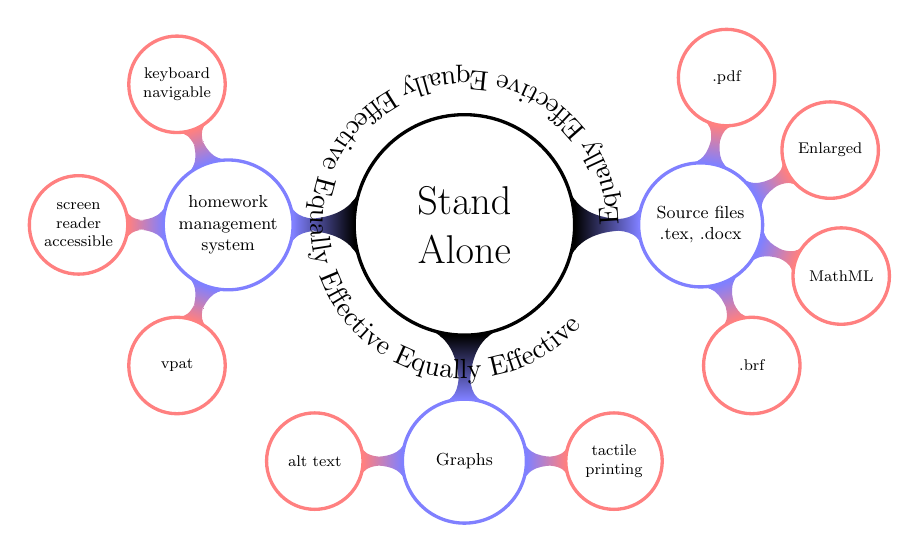
\begin{tikzpicture}[mindmap,
         concept/.append style={fill={none}},
         root concept/.style={concept color=blue},
         level 1 concept/.append style=
         {every child/.style={concept color=blue!50},level distance = 30mm},
         level 2 concept/.append style=
         {every child/.style={concept color=red!50},level distance = 19mm},
         every node/.append style={align=center,scale=0.7},
      ]
      \node [concept,font=\huge] {Stand\\ Alone}
      child[grow=0, visible on=<2->] {node[concept] {Source files .tex, .docx}
         child[grow=80, visible on=<2->]{node[concept] {.pdf}}
         child[grow=30, visible on=<2->]{node[concept] {Enlarged}}
         child[grow=-20, visible on=<2->]{node[concept] {MathML}}
         child[grow=-70, visible on=<2->]{node[concept] {.brf}}
      }
      child[grow=-90,visible on=<3->] {node[concept] {Graphs}
         child[grow=0,visible on=<3->]{node[concept] {tactile printing}}
         child[grow=180,visible on=<3->]{node[concept] {alt text}}
      }
      child[grow=180,visible on=<4->] {node[concept] {homework management system}
         child[grow=110,visible on=<4-> ] {node[concept] {keyboard navigable}}
         child[grow=180,visible on=<4->] {node[concept] {screen reader accessible}}
         child[grow=250,visible on=<4->] {node[concept] {vpat}}
      };
      \node at (0,0) [inner sep=9mm,decorate,circle,decoration=
      {text along path,text={Equally Effective Equally Effective Equally Effective  Equally Effective }}] {};
      %\draw decorate[decoration={text along path,text={Equally Effective}}]
      %{(-3,0) arc (135:45:.5cm)};

   \end{tikzpicture}
\end{frame}

\begin{frame}[c]{What stands alone?}
   % Which content creation tools stand alone?
   \pause
   \begin{columns}
      \begin{column}[c]{.33\textwidth}
         \tikz \node[fill=green!20,draw=green, rounded corners,very thick,inner sep=0mm]{%
            \vbox{%
               \begin{itemize}
                  \item MS Word with MathType
                  \item \LaTeX
                  \item LibreOffice
                  \item Scientific Notebook
                  \item Graphs
                  \item Prepared lecture notes
                  \item Desire2Learn
                  \item WeBWorK
                  \item Videos
               \end{itemize}
            }%
         };
      \end{column}%
      \pause
         \begin{column}[c]{.33\textwidth}
            \tikz \node[fill=orange!20,draw=orange, rounded corners,very thick,inner sep=0mm]{%
               \vbox{%
                  \begin{itemize}
                     \item[] MyMathLab
                  \end{itemize}
               }
            };
            \vfill
         \end{column}%
      \pause
         \begin{column}[c]{.33\textwidth}
            \tikz \node[fill=red!20,
               draw=red,
               rounded corners,
               very thick,
               inner sep=0mm,
               %decorate,decoration={zigzag,segment length=10mm,amplitude=2.0mm},
            ]{%
               \vbox{%
                  \begin{itemize}
                     \item MS Word OMML
                     \item PowerPoint
                     \item TestGen
                     \item GeoGebra applets
                     \item Flash-based applets
                     \item Other media
                  \end{itemize}
               }
            };
         \end{column}
   \end{columns}

\end{frame}


\begin{frame}[fragile]{Collaboration is key}
   \makebox[\textwidth][c]{%
      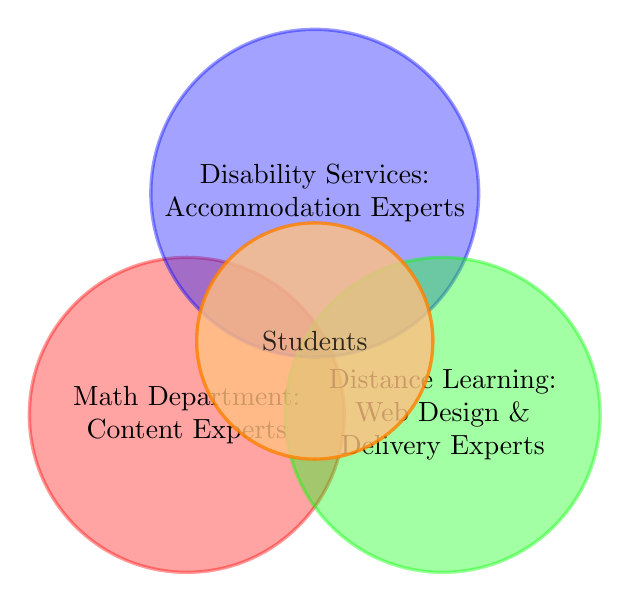
\begin{tikzpicture}[venn circle/.style={draw=#1,
               circle,
               very thick,
               minimum width=4cm,
               text=black,
               fill=#1!90,
               opacity=0.4,
               text opacity=1},
         every node/.append style={align=center}]
         \node [venn circle = red] (A) at (0,0) {Math Department:\\ Content Experts};
         \visible<2->{\node [venn circle = blue] (B) at (60:3.25cm) {Disability Services:\\ Accommodation Experts};}
         \visible<3->{\node [venn circle = green] (C) at (0:3.25cm) {Distance Learning:\\ Web Design \&\\Delivery Experts};}
         \visible<4->{\node[circle,fill=orange!50,draw=orange,very thick,opacity=0.8,minimum width=3cm] at (barycentric cs:A=1/3,B=1/3,C=1/3 ){Students};}
      \end{tikzpicture}
   }
\end{frame}
